\chapter{Manual del usuario}
\label{anexo:manualUsuario}

\section{Verificaciones iniciales}
\label{anexo:verificaciones}
Antes de poner en funcionamiento la planta verifique cada uno de los siguientes
items:

\tcbset{before app=\parfillskip 0pt}
\begin{tcolorbox}[title=Nivel de agua]
\textbf{Tanques vacíos:} llene con agua cada uno de los tanques hasta un 55\%
del total de su capacidad aproximadamente.

\textbf{Tanques con agua:} verifique que cada uno de los tanques no esté por
encima del 80\% ni por debajo del 20\%.

\end {tcolorbox}
\begin{lattention}
En \textbf{modo automático}, si el nivel del tanque controlado desciende por
debajo del 20 \% o aumenta por encima del 80\% se detiene la planta 
automáticamente. Puede transvasar el fluido de un tanque a otro utilizando el
modo manual del \gls{scada} (ver Sec. \ref{anexo:operacionSCADA} del Manual
del Usuario) o encendiendo
manualmente las electrobombas (ver Sec. \ref{anexo:motoresManual} del Manual del
Usuario).

La planta no podrá volver a encenderse en modo automático hasta que se confirme
por parte del usuario que la planta no está en estado de emergencia (mediante el
\gls{scada} o poniendo a 1 la bandera \verb|MW1:X7|).
\end{lattention}

\begin{tcolorbox}[title=Válvulas manuales, breakable]

La planta cuenta con 6 válvulas manuales (Ver \gls{pyid}).
%Se describirá la posición de cada una
%de ellas para un correcto funcionamiento de la planta.

 \begin{itemize}
  \item \textbf{Purgado de los tanques:} completamente cerradas.
  \item \textbf{Ecualización de la planta:}
  \begin{itemize}
   \item Sin tiempo muerto: \verb|VM2| debe estar abierta $2$ vueltas, y
   \verb|VM1| debe cerrarse hasta que el manómetro \verb|PI 1| indique
   $0.4\,kg/cm^2$.
   \item Con tiempo muerto: \verb|VM2| debe estar abierta $1.5$ vueltas, y
   \verb|VM1| debe cerrarse hasta que el manómetro \verb|PI 1| indique
   $0.5\,kg/cm^2$.
  \end{itemize}
  \item \textbf{Tiempo muerto \texttt{VDT}:} abierta si se desea trabajar con
la planta sin tiempo muerto, cerrada si se desea trabajar con tiempo muerto.
  \item \textbf{Perturbación \texttt{VMP}:} totalmente cerrada inicialmente.
 \end{itemize}
 \tcblower
 \textbf{Nota:} estas válvulas están presentes para modificar el sistema y
generar distintos
escenarios en la planta. Al modificar las características del sistema se deben
ajustar los valores del controlador.
\end {tcolorbox}

\begin{tcolorbox}[title=Presión de aire en la válvula]
  Asegúrese que la presión de aire esté regulada a $4\,bar$. Se debe controlar
  el correcto funcionamiento del filtro y regulador, realizando purgas en caso
de ser necesario.
 \tcblower
  \textbf{Nota:} un filtro regulador se utiliza de la siguiente manera:
 \begin{enumerate}
    \item Desconectar la tubería flexible de aire al electroposicionador.
    \item Se conecta la línea de aire comprimido al regulador.
    \item Se visualiza el valor de presión en el manómetro
    \item Se desplaza hacia arriba la maneta de regulación y se gira hasta
      alcanzar el valor de presión deseado.
    \item Se vuelve la maneta de regulación a su posición original.
    \item Conectar nuevamente la tubería flexible de aire al
electroposicionador.
 \end{enumerate}
\end {tcolorbox}
%\todo{agregar filtro de aire}

\begin{lattention}
Nunca conectar la linea de aire comprimido de manera directa al
electroposicionador,
sin el filtro regulador.
Puede dañarlo de manera irreversible si la presión de aire
supera los $7\,bar$.
\end{lattention}

\begin{tcolorbox}[title=Motores]
Para poder encender los motores se debe verificar que no están trabados.
Para ello, se recomienda retirar la jaula que recubre los ventiladores
de los motores y hacerlos girar manualmente.
\end {tcolorbox}

\begin{lattention}
Solo conecte la planta a la red eléctrica ($220\,V$, corriente alterna) luego 
de haber realizado todas las verificaciones antes mencionadas. 
\end{lattention}

\section{Activación manual de los motores}
\label{anexo:motoresManual}
Se explican a continuación los pasos a seguir para activar, de modo manual, los
motores de la planta.
 \begin{lattention}
 La activación manual de los motores debe utilizarse exclusivamente en el caso
de que el sistema SCADA no responda.
Por favor, en caso de dudas consulte con el encargado del laboratorio.
\end{lattention}

%   \begin{enumerate}
%    \item Controlar que no estén trabados.
%    \item Energizar el sistema.
%    \item Conectar el aire, presión 4 bares.
%    \item Activar el relé manualmente que sea necesario.
%   \end{enumerate}

\begin{table}[H]
\centering
\renewcommand*{\arraystretch}{0.01}
\begin{tabular}{*{2}{m{0.435\textwidth}}}
\hline
% Fernando: para mi es más importante esto que conectar la presión de aire.
% No se puede abrir la válvula así que no sirve de nada conectarla.
  Controlar que las electrobombas no estén bloqueadas.
  &\begin{center}
    %\rule{0.4\textwidth}{0.3\textwidth}
    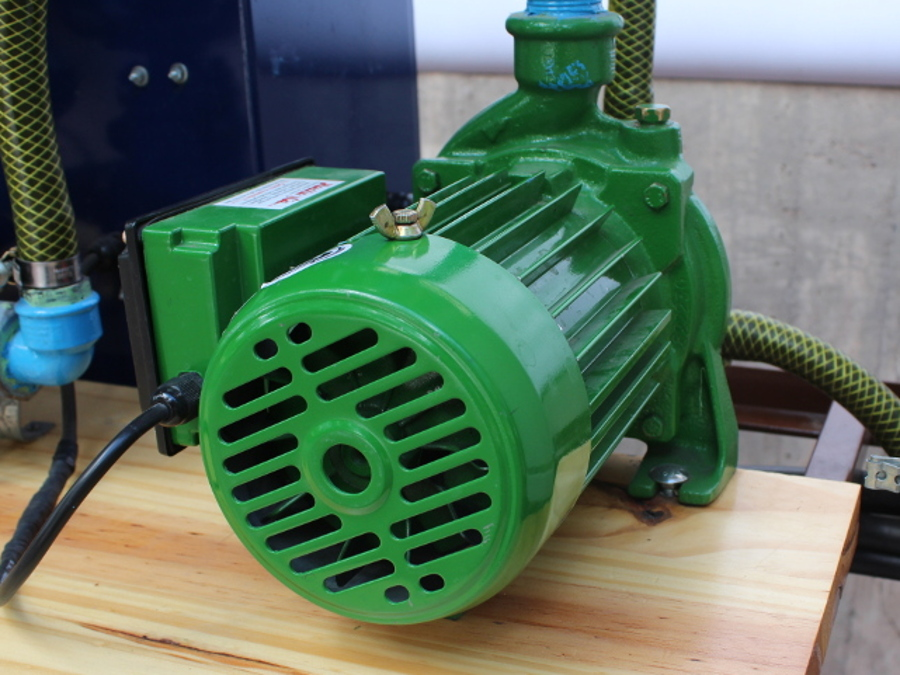
\includegraphics[width=0.4\textwidth]
      {Anexos/images/bombaBottom.JPG}
  \end{center}\\
\hline
    Energizar el sistema. Activar el interruptor termomagnético ubicado dentro
    del tablero eléctrico.
    &\begin{center}
      %\rule{0.4\textwidth}{0.3\textwidth}
      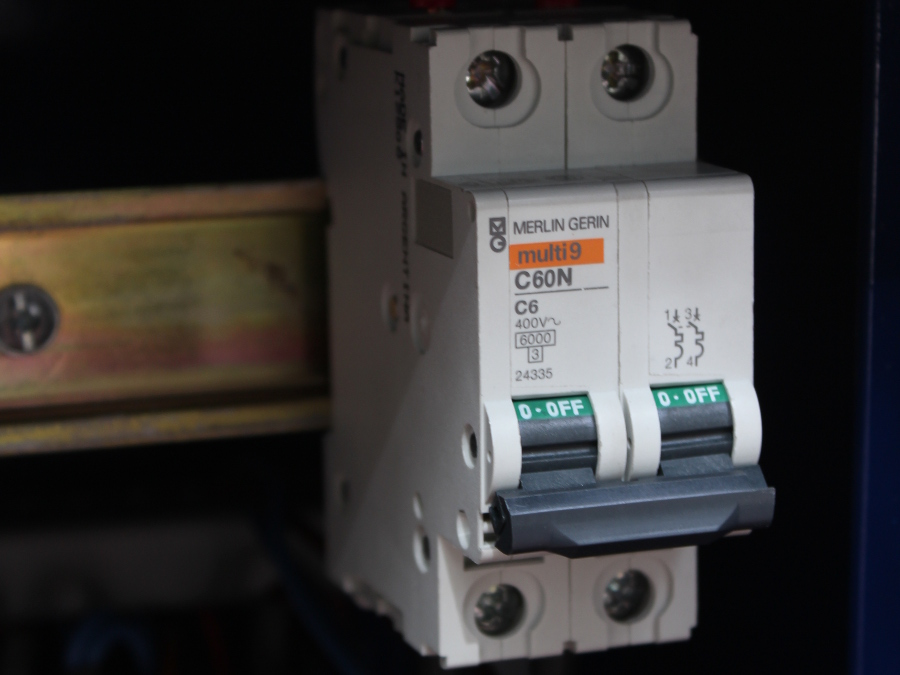
\includegraphics[width=0.4\textwidth]
	{Anexos/images/disyuntor.JPG}
    \end{center}\\
\hline
    Activar manualmente el relé de la electrobomba correspondiente.
    En la imagen se
    puede apreciar la llave (color verde claro) que debe accionarse. Para mas 
    información acerca del relé utilizado en esta planta, refiérase a la
    hoja de datos del mismo.
    &\begin{center}
      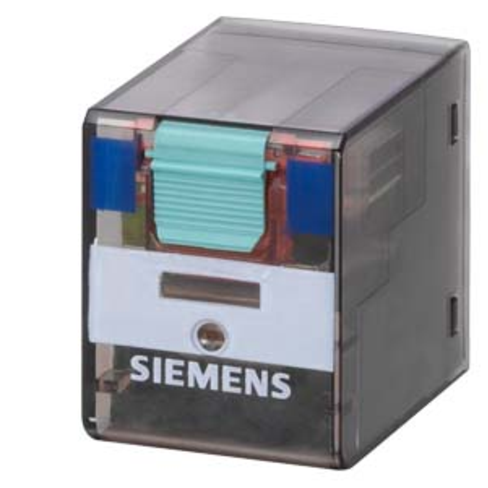
\includegraphics[width=0.3\textwidth]{Anexos/images/rele.pdf}
    \end{center}\\
\hline
\end{tabular}
\end{table}
